\documentclass[twoside,10pt,a4paper]{article}
\usepackage[utf8]{inputenc}
\usepackage[english]{babel}
\usepackage{amsmath}
\usepackage{amsfonts}
\usepackage{amssymb}
\usepackage{graphicx}

\usepackage[left=2cm,right=2cm,top=2cm,bottom=3cm]{geometry}
\usepackage{fancyvrb}
\usepackage{listings}
\usepackage{xparse}
\usepackage{tikz} % ajout de dessins LaTeX
\usepackage{graphicx}
\usepackage{float}  % alignement des figures
\usepackage{fancyhdr}
\usepackage{enumitem}
\usepackage{verbatim}
\usepackage{xcolor}

\usepackage{caption}
\usepackage{subcaption}

\pagestyle{fancy} %fancyhdr
	\fancyhf{} %fancyhdr
	\renewcommand{\sectionmark}[1]{\markboth{#1}{}}
	\fancyhead[R]{NLDCI Set 7 Solutions} %INSERT TITLE HERE FOR fancyhdr
	\fancyhead[L]{\nouppercase{\leftmark}} %fancyhdr
	\cfoot{\thepage} %fancyhdr
	\setlength{\headheight}{35pt}
	\setlength{\parindent}{0pt}

\begin{titlepage}
\title{\huge \textbf{Nonlinear Dynamics \& Chaos I \\ \Large Exercice Set 7 Solutions}}	%TITLE
\author{ }		%AUTHOR
\date{ }	%DATE

\end{titlepage}

	\definecolor{MyBlue}{HTML}{4A90E2}
	\definecolor{MyRed}{HTML}{D0021B}
	\definecolor{MyGreen}{HTML}{7ED321} % Same color use in Mathcha


\begin{document}

\maketitle

\section*{Question 1}
Consider a planar Hamiltonian system
\begin{align*}
	\dot{x} &= \frac{\partial H(x,y)}{\partial y} + f_1(x,y), \\
	\dot{y} &= - \frac{\partial H(x,y)}{\partial x} + f_2(x,y),
\end{align*}
where the twice continuously differentiable function $H(x,y)$ is the Hamiltonian associated with the system (say, the energy in classical mechanics, or the stream function in fluid mechanics), and the continuously differentiable $\mathbf{f} = (f_1, f_2)$ is a dissipative term (say, damping in classical mechanics, or compressible terms in fluid mechanics). Assume that $\nabla \cdot \mathbf{f} \neq 0$ for all $(x,y) \in \mathbb{R}^2$. (Linear damping, for instance has this property.)

Show that the above system can have no limit cycles.

\section*{Solution 1}
\begin{equation}
	\begin{bmatrix}\label{S05E011}
		\dot{x} \\
		\dot{y}
	\end{bmatrix} =
	\underline{F}(x,y) := \begin{bmatrix}
		\displaystyle \frac{\partial H}{\partial y}(x,y) + f_1(x,y) \\
		\displaystyle -\frac{\partial H}{\partial x}(x,y) + f_2(x,y)
	\end{bmatrix}
\end{equation}
\begin{align*}
	\text{div}(\underline{F}) &= \frac{\partial^2 H}{\partial x \partial y}(x,y) + \frac{\partial f_1}{\partial x}(x,y) - \frac{\partial^2 H}{\partial y \partial x}(x,y) + \frac{\partial f_2}{\partial y} \\
	&= \text{div}(\underline{f}) \qquad (H \in C^2) \\
	&\neq 0 \quad \forall (x,y)\in \mathbb{R}^2
\end{align*}
Thus, by the Bendixson's criterion, (\ref{S05E011}) does not have a periodic solution in $\mathbb{R}^2$.

\newpage

\section*{Question 2 - Accuracy of averaging}
Show that on time scales of $\mathcal{O}(1/\varepsilon)$, a solution $\mathbf{x}(t)$ with $\mathbf{x}(0) = \mathbf{x}_0$ of the dynamical system
\begin{equation}\label{Q01E01}
	\dot{\mathbf{x}} = \varepsilon \mathbf{f}(\mathbf{x},t, \varepsilon), \qquad \mathbf{x} \in \mathbb{R}^n,
\end{equation}
($\varepsilon$ is a small parameter and $\mathbf{f}$ is a smooth function that is $T$-periodic in time) remains $\mathcal{O}(\varepsilon)$-close to any solution $\mathbf{y}(t)$ with $\mathbf{y}(0) = \mathbf{x}_0 + \mathcal{O}(\varepsilon)$ of the averaged system
\begin{equation}\label{Q01E02}
	\dot{\mathbf{y}} = \varepsilon \bar{\mathbf{f}}_0 (\mathbf{y}), \qquad \mathbf{y} \in \mathbb{R}^n,
\end{equation}
where
\begin{equation*}
	\bar{\mathbf{f}}_0 (\mathbf{y}) = \frac{1}{T} \int_0^T f(y,t,0) \, \text{d}t.
\end{equation*}
\textit{Hint}: Subtract (\ref{Q01E02}) from (\ref{Q01E01}) and integrate to obtain an expression for $|\mathbf{x}(t) - \mathbf{y}(t)|$. Estimate $|\mathbf{x}(t) - \mathbf{y}(t)|$ from above using the facts that $\bar{\mathbf{f}}$ is Lipschitz and $|\hat{f} - \bar{f}|/\varepsilon$ is uniformly bounded, where $\hat{f}$ is the right-hand-side of the system into which (\ref{Q01E01}) is transformed by the averaging transformation $\mathbf{x} = \mathbf{y} + \varepsilon \mathbf{w}(\mathbf{y},t)$. Then use the following generalized Gronwall inequality:

If $u(t), v(t), c(t)$ are non-negative functions, $c(t)$ is differentiable, and
\begin{equation*}
	v(t) \leq c(t) + \int_0^t u(s)v(s) \, \text{d}s,
\end{equation*}
then
\begin{equation*}
	v(t) \leq c(0) e^{\int_0^t u(s)\, \text{d}s} + \int_0^t c'(s)e^{\int_s^t u(\tau)\,\text{d}\tau}\, \text{d}s.
\end{equation*}

\section*{Solution 2}
Remember from the lecture on averaging that $\dot{x} = \varepsilon f(x,t, \varepsilon)$ can be transformed to the differential equation
\begin{equation}\label{S05E021}
	\dot{\tilde{x}} = \varepsilon \bar{f}_0(\tilde{x}) + \varepsilon^2f_1(\tilde{x},t,\varepsilon)
\end{equation}
Through the near-identity transformation $x = \tilde{x} + \varepsilon w(\tilde{x},t)$.

Moreover, $f_1$ is globally bounded, i.e., there exists $L_1 > 0$ such that
\begin{equation*}
	|f_1(\tilde{x},t,\varepsilon)| < L_1 \qquad \forall t > 0 \text{ and } \forall \tilde{x}\in \mathbb{R}^n
\end{equation*}
Now by construction $|x(t) - \tilde{x}(t)| = \varepsilon|w(\tilde{x}(t),t)| = \mathcal{O}(\varepsilon)$
Therefore, it suffices to show that solutions of the averaged equation
\begin{equation}\label{S05E022}
	\dot{y} = \varepsilon \bar{f}_0(y)
\end{equation}
remain $\mathcal{O}(\varepsilon)$ close to the solutions of (\ref{S05E021}).

Subtracting (\ref{S05E022}) from (\ref{S05E021}), integrating and dropping the tilde (\textasciitilde) sign, we get 
\begin{equation*}
	x(t) - y(t) = x_0 - y_0 + \varepsilon \int_0^t \left( \bar{f}_0(x(s)) - \bar{f}_0(y(s)) \right) \, \text{d}s + \varepsilon^2 \int_0^t f_1(x(s),s,\varepsilon) \, \text{d}s
\end{equation*}
\begin{equation*}
	\Longrightarrow |x(t) - y(t)| \leq |x_0 - y_0| + \varepsilon \int_0^t L_2|x(s) - y(s)|\,\text{d}s + \varepsilon^2 \int_0^t L_1 \,\text{d}s
\end{equation*}
where we used boundedness of $f_1$ and Lipschitz continuity of $\bar{f}_0$:
\begin{equation*}
	|f_0(x) - f_0(y)| \leq L_2 |x - y|
\end{equation*}
Therefore,
\begin{equation}\label{S05E023}
	|x(t) - y(t)| \leq |x_0 - y_0| + \varepsilon^2 L_1t + \int_0^t \varepsilon L_2 |x(s) - y(s)|\,\text{d}s
\end{equation}
Now apply Gronwall's inequality with $v(t) = |x(t) - y(t)|$, $u(t) = \varepsilon L_2$ and $c(t) = |x_0 - y_0| + \varepsilon^2 L_1t$ to get
\begin{align*}
	|x(t) - y(t)| &\leq |x_0 - y_0|e^{\varepsilon L_2 t} + \int_0^t \varepsilon L_1 e^{\varepsilon L_2 (t-s)}\,\text{d}s \\
	&= |x_0 - y_0|e^{\varepsilon L_2 t} + \varepsilon \frac{L_1}{L_2} \left( e^{\varepsilon L_2 t} -1 \right) \leq \left[ |x_0 - y_0| + \varepsilon \frac{L_1}{L_2} \right] e^{\varepsilon L_2 t}
\end{align*}
Since $|x_0 - y_0| = \mathcal{O}(\varepsilon)$, we conclude that $|x(t) - y(t)|= \mathcal{O}(\varepsilon)$ as long as $t\in \left[0,\frac{1}{\varepsilon L_2}\right)$, i.e., time scales of $\mathcal{O}(1/\varepsilon)$.

\newpage

\section*{Question 3 - Unsteady separation in time-periodic fluid flows}
Fluid trajectories $\mathbf{x}(t) = (x(t),y(t))$ in a two-dimensional time-periodic flow satisfy the differential equations
\begin{equation}\label{Q03E01}
	\begin{aligned}
		\dot{x} &= u(x,y,t), \qquad u(x,y,t) = u(x,y,t+T), \\
		\dot{y} &= v(x,y,t), \qquad v(x,y,t) = v(x,y,t+T),
	\end{aligned}
\end{equation}
where $T>0$ is the period, $u$ and $v$ are smooth velocity components satisfying the incompressibility condition $u_x + v_y \equiv 0$. Assume that the fluid is bounded by a wall at $y=0$, on which the velocity field satisfies the no-slip boundary conditions $u(x,0,t) = v(x,0,t)=0$. As a result, all boundary points are nonhyperbolic fixed points for (\ref{Q03E01}).

We say that a boundary point $\mathbf{p}_0 = (x_0,0)$ is a separation point for the flow (\ref{Q03E01}) if $\mathbf{p}_0$ admits an unstable manifold $W^u(\mathbf{p}_0)$. Physically, $W^u(\mathbf{p}_0)$ is a time-dependent curve of fluid particles that shrinks to $\mathbf{p}_0$ is backward time. In forward time, $W^u(\mathbf{p}_0)$ attracts fluid particles, then ejects them from the vicinity of the wall (see Fig. 1). Show that separation points satisfy the criteria
\begin{equation*}
	\int_0^T u_y(x_0,0,t) \, \text{d}t = 0, \quad \int_0^T v_{yy}(x_0,0,t)\, \text{d}t > 0,
\end{equation*}
i.e., separation takes place where the average of the wall-shear is zero and the average of $v_{yy}$ is positive.

\textit{Hint}: Use incompressibility and the boundary conditions to show that (\ref{Q03E01}) can be rewritten as
\begin{align*}
	\dot{x} &= yU(x,y,t), \\
	\dot{y} &= y^2V(x,y,t).
\end{align*}
To focus on the vicinity of the boundary, introduce the scaled variable $y=\varepsilon \eta$, where $0 \leq \varepsilon \ll 1$. Show that the resulting $(\dot{x},\dot{\eta})$ equations are slowly varying and find the corresponding averaged equations. For the averaged equations, rescale time on trajectories by letting $\frac{d\tau}{dt} = \eta(t)$ in order to remove the common $\eta$ factor from the right-hand-side, and look for a hyperbolic fixed point with an unstable manifold off the wall. Use the averaging theorem to relate your results to the original system (\ref{Q03E01}).

\begin{figure}[H]
	\centering
	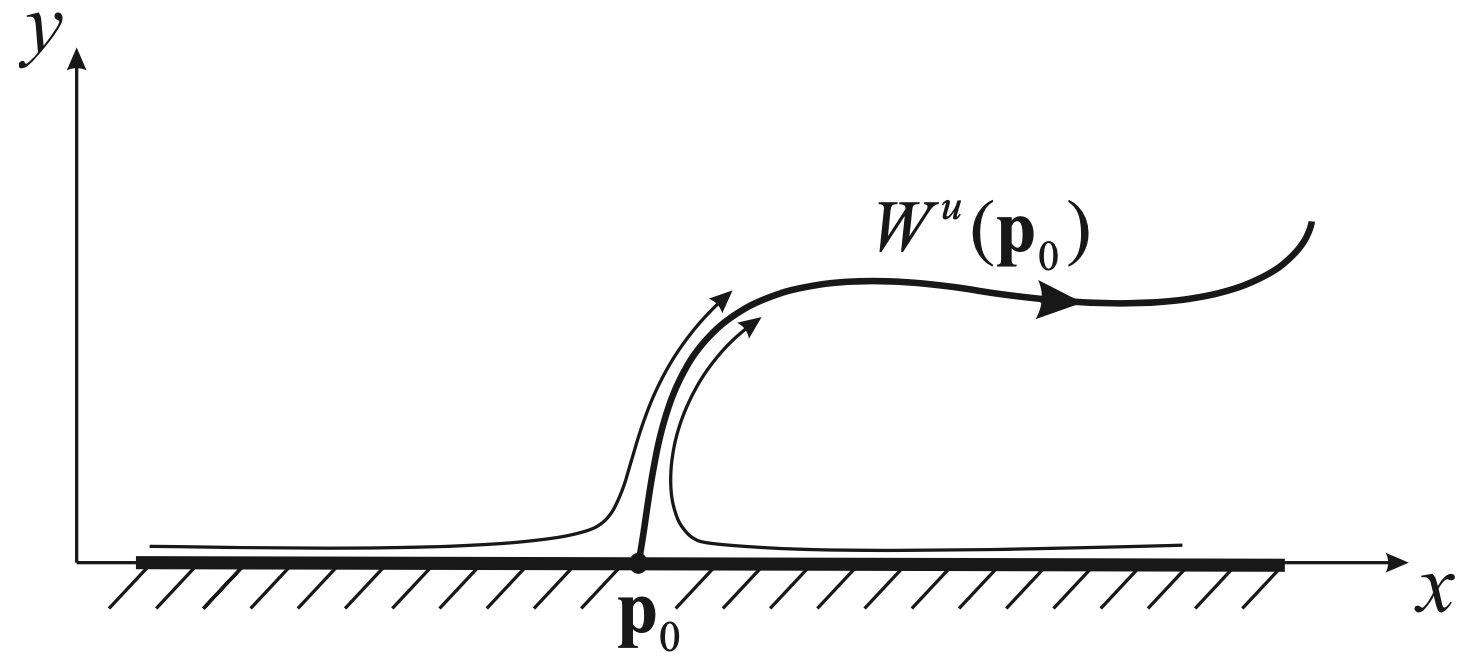
\includegraphics[scale=0.15]{Graphics/Q03D01.png}
	\caption{Unsteady separation from a no-slip wall}
\end{figure}

\section*{Solution 3}
We start with the Taylor expansions of $u(x,y,t)$ and $v(x,y,t)$ in $y$ near $y=0$:
\begin{equation}\label{S05E031}
	\begin{cases}
		\displaystyle u(x,y,t) = u(x,0,t) + \frac{\partial u}{\partial y}(x,0,t)y + \mathcal{O}(|y|^2) \\
		\displaystyle v(x,y,t) = v(x,0,t) + \frac{\partial v}{\partial y}(x,0,t)y + \frac{1}{2} \frac{\partial^2 v}{\partial y^2}(x,0,t)y^2 + \mathcal{O}(|y|^3)
	\end{cases}
\end{equation}
But $u(x,0,t) = v(x,0,t) = 0$ for any $x$.

Differentiating $u(x,0,t) = 0$ with respect to $x$ we get $\displaystyle \frac{\partial u}{\partial x}(x,0,t) = 0$.

By incompressibility:
\begin{align*}
	\frac{\partial u}{\partial x} &= - \frac{\partial v}{\partial y} \\
	\Longrightarrow \frac{\partial v}{\partial y}(x,0,t) &= - \frac{\partial u}{\partial x}(x,0,t) = 0, \;\; \forall x
\end{align*}
Hence (\ref{S05E031}) simplifies to
\begin{equation*}
	\begin{cases}
		\displaystyle u(x,y,t) = \frac{\partial u}{\partial y}(x,0,t)y + \mathcal{O}(|y|^2) = y U(x,y,t) \\
		\displaystyle v(x,y,t) = \frac{1}{2} \frac{\partial^2 v}{\partial y^2}(x,0,t)y^2 + \mathcal{O}(|y|^3) = y^2V(x,y,t)
	\end{cases}
\end{equation*}
Also note that
\begin{equation}\label{S05E032}
	\begin{cases}
		\displaystyle U(x,y,t) = \frac{\partial u}{\partial y}(x,0,t) \\
		\displaystyle V(x,y,t) = \frac{1}{2}\frac{\partial^2 v}{\partial y^2}(x,0,t)
	\end{cases}
\end{equation}
\begin{center}
	\color{red} Higher-order terms are identically zero
\end{center}
Therefore,
\begin{equation*}
	\begin{cases}
		\dot{x} = yU(x,y,t) \\
		\dot{y} = y^2V(x,y,t)
	\end{cases}
\end{equation*}
Scaling $y$ as $y = \varepsilon \eta$, we get:
\begin{equation}\label{S05E033}
	\begin{cases}
		\dot{x} = \varepsilon \eta U(x,\varepsilon \eta, t) \\
		\dot{\eta} = \varepsilon \eta^2 V(x, \varepsilon \eta,t)
	\end{cases}
\end{equation}
Since $U$ and $V$ are also $T$-periodic, averaging theory applies to (\ref{S05E033}) with the averaged equations
\begin{equation}\label{S05E034}
	\begin{cases}
		\dot{x} = \varepsilon \eta \bar{U}(x) \\
		\dot{\eta} = \varepsilon \eta^2 \bar{V}(x)
	\end{cases}
\end{equation}
where
\begin{equation}\label{S05E035}
	\begin{cases}
		\displaystyle \bar{U}(x) = \frac{1}{T} \int_0^T U(x,0,s)\,\text{d}s = \frac{1}{T} \int_0^T \frac{\partial u}{\partial y}(x,0,s)\,\text{d}s \\
		\displaystyle \bar{V}(x) = \frac{1}{T} \int_0^T V(x,0,s)\,\text{d}s = \frac{1}{2T} \int_0^T \frac{\partial^2 v}{\partial y^2}(x,0,s)\,\text{d}s
	\end{cases}
\end{equation}

Rescaling time as $\displaystyle \frac{d\tau}{dt}=\eta(t)$ and denoting the derivative with respect to $\tau$ by prime sign ($'$) we get
\begin{equation*}
	\dot{x} = \frac{dx}{dt} = \frac{dx}{d\tau}\frac{d\tau}{dt} = \eta x' \quad , \quad \dot{\eta}= \eta \eta'
\end{equation*}

Substituting these expressions in (\ref{S05E035}), we get
\begin{equation}\label{S05E036}
	\begin{cases}
		x' = \varepsilon \bar{U}(x) \\
		\eta' = \varepsilon \eta \bar{V}(x)
	\end{cases}
\end{equation}

Equation (\ref{S05E036}) has a fixed point $(x_0, \eta=0)$ on the wall if and only if $\bar{U}(x_0,0)=0$. Using (\ref{S05E035}), we have
\begin{equation}\label{S05E037}
	\bar{U}(x_0) = 0 \Longleftrightarrow \boxed{\int_0^T \frac{\partial u}{\partial y}(x_0,0,s)\,\text{d}s = 0}
\end{equation}

Now we turn to the stability of the fixed point $(x_0,0)$ on the wall by linearising (\ref{S05E036}) around this fixed point:
\begin{equation*}
	\underline{\xi}' = \varepsilon \underbrace{\begin{pmatrix}
		\displaystyle \frac{\partial \bar{U}}{\partial x}(x_0) & 0 \\
		0 & \displaystyle \bar{V}(x_0)
	\end{pmatrix}}_{:=A} \underline{\xi}
\end{equation*}

The matrix $A$ has eigenvalues $\displaystyle \varepsilon \frac{\partial \bar{U}}{\partial x}(x_0)$ and $\varepsilon \bar{V}(x_0)$ corresponding to eigenvectors $\displaystyle \begin{pmatrix} 1 \\ 0 \end{pmatrix}$ and $\displaystyle \begin{pmatrix} 0 \\ 1 \end{pmatrix}$ respectively.

For the unstable manifold to be off the wall, we need $\bar{V}(x_0)>0$.

Using (\ref{S05E035}), we have
\begin{equation}\label{S05E038}
	\bar{V}(x_0) > 0 \Longleftrightarrow \boxed{\int_0^T \frac{\partial^2 v}{\partial y^2}(x_0,0,s)\,\text{d}s > 0}
\end{equation}

\subsection*{Exercice:}
Show that
\begin{equation*}
	\frac{\partial \bar{U}}{\partial x}(x_0) = -2 \bar{V}(x_0)
\end{equation*}
and hence $(x_0,0)$ is a hyperbolic fixed point of (\ref{S05E036}) given condition (\ref{S05E038}) holds.

The conditions (\ref{S05E037}) and (\ref{S05E038}) together imply that there exists a hyperbolic fixed point of the averaged system (\ref{S05E036}).

The theory of averaging guarantees, the existence of a fixed point $(x_0^\varepsilon,0)$ of the original time-periodic flow which is $\mathcal{O}(\varepsilon)$ close to the fixed point $(x_0^\varepsilon,0)$ of the averaged system.

Moreover, $(x_0^\varepsilon,0)$ has an unstable manifold $W_\varepsilon^{\text{u}} \;\; \mathcal{O}(\varepsilon)$-close to $W^{\text{u}}$ of the averaged system.

\subsection*{Remark:}
A hyperbolic fixed point of the averaged system, in general, signals a nearby limit cycle of the original system. But, in the above example, it signals a fixed point of the original system since the points on the wall don't move due to the no-slip boundary condition.


\newpage

\section*{Solution 4}
Consider the 1D equation
\begin{equation*}
	\dot{x} = \varepsilon (-x + \sin^2(t) + \varepsilon \cos^2(t))
\end{equation*}
Using averaging, determine which statement is correct.

\begin{enumerate}[label=(\alph*)]
	\item $x = 0$ is an attracting fixed point.
	\item $\displaystyle x = \frac{1}{2}$ is an attracting fixed point.
	{\color{MyRed}\item There exists an attracting periodic orbit close to $\displaystyle x = \frac{1}{2}$.}
\end{enumerate}

{\color{MyRed}
Let
\begin{equation*}
	f(x,t; \varepsilon) = -x + \sin^2(t) + \varepsilon \cos^2(t)
\end{equation*}
\begin{align*}
	\bar{f} &= \frac{1}{\pi} \int_0^\pi f(x,t; \varepsilon) \; \text{d}t \\
	&= -x + \frac{1}{2}
\end{align*}
Averaged flow:
\begin{equation*}
	\dot{x} = \varepsilon \left( -x + \frac{1}{2} \right)
\end{equation*}
}

\section*{Solution 5}
Which system can be treated by averaging ? Assume that $0 < \varepsilon \ll 1$.

\begin{enumerate}[label=(\alph*)]
	\item $ \ddot{x} + 4x = \varepsilon(1 + x e^t) $
	\item $ \displaystyle \begin{cases}
		\dot{x} = \varepsilon y \sin(t) \\
		\dot{y} = x \cos(\sqrt{2}t)
	\end{cases} $
	{\color{MyRed}\item $ \displaystyle \begin{cases}
		\dot{x} = \varepsilon x^4 \\
		\dot{y} = \varepsilon(x + \sin^2(t))
	\end{cases} $}
	\item None of the above
\end{enumerate}

\section*{Solution 6}
Consider the dynamical system $ \dot{x} = A(t)x $ with
\begin{equation*}
	A(t) = {\renewcommand*{\arraystretch}{1.25}\begin{pmatrix}
		\displaystyle -1 + \frac{3}{2}\cos^2(t) & \displaystyle 1 - \frac{3}{2} \sin(t)\cos(t) \\
		\displaystyle -1 - \frac{3}{2} \sin(t)\cos(t) & \displaystyle -1 + \frac{3}{2} \sin^2(t)
	\end{pmatrix}}
\end{equation*}
Which of the following statements is correct?

\begin{enumerate}[label=(\alph*)]
	\item The eigenvalues of $A(t)$ are $\displaystyle \lambda_{1,2} = \frac{1}{4}(-1 \pm i\sqrt{7})$. Therefore the $x = 0$ fixed point is stable.
	\item The eigenvalues of $A(t)$ are $\displaystyle \lambda_{1,2} = \frac{1}{4}(-1 \pm i\sqrt{7})$. Therefore the $x = 0$ fixed point is asymptotically stable.
	\item The eigenvalues of $A(t)$ are $\displaystyle \lambda_{1,2} = \pm \frac{i}{2}\cos(2t)$. Therefore the stability of the $x = 0$ cannot be determined.
	{\color{MyRed}\item None of the above}
\end{enumerate}

{\color{MyRed} The stability of time-dependent systems cannot be determined by the eigenvalues of $A(t)$.

Moreover, $\text{Tr}(A(t)) = -2 + \frac{3}{2} = - \frac{1}{2}$ so the stability cannot be determined by Liouville's theorem either.}

\section*{Solution 7}
Does the classic theory of averaging apply to the dynamical system given below?
\begin{equation*}
	\ddot{x} = \varepsilon f(x,t), \quad f(x, t + T) = f(x,t), \quad x \in \mathbb{R}^n
\end{equation*}

\begin{enumerate}[label=(\alph*)]
	\item Yes, after the introduction of the new variable $y = \dot{x}$.
	\item Yes, but only for $ 0 \leq |\varepsilon| \ll 1 $.
	\item Yes, but only for $n = 1$.
	{\color{MyRed}\item None of the above}
\end{enumerate}

{\color{MyRed}In general, averaging applies to $\dot{x} = \varepsilon f(x,t; \varepsilon); \; f(x,t+T; \varepsilon) = f(x,t;\varepsilon)$.
}

\section*{Solution 8}
Consider the gradient dynamical system:
\begin{equation*}
	\dot{x} = -\nabla V(x)
\end{equation*}
Where $V: \mathbb{R}^n \longrightarrow \mathbb{R}, \; V \in C^1, \; n \geq 2$. Which of the following statements are true?

\begin{enumerate}[label=(\alph*)]
	\item This system cannot have a limit cycle in a region where $\Delta V$ has constant sign.
	{\color{MyRed}\item This system cannot have a limit cycle, because $ V(x(t)) $ is monotone decreasing in $t$.}
	\item The system can only have stable limit cycles because of the negative sign in front of $\nabla V(x)$.
	\item None of the above
\end{enumerate}

{\color{MyRed}
	If $x(t) = \gamma(t)$ was a limit cycle with $\gamma(t) = \gamma(t + T)$, then $V(\gamma(t)) = V(\gamma(t + T))$. But
	\begin{equation*}
		\frac{d}{dt} V(x(t)) = - ||\nabla V(x) ||^2 \leq 0.
	\end{equation*}
	Thus, $V(x(t))$ is monotone decreasing in t and, we cannot have a periodic solution.
}







\end{document}